\documentclass[french]{extarticle}
\usepackage{rapport/lib/algorithmeUTF8}
\usepackage[utf8]{inputenc}
\usepackage[top=2.5cm, bottom=2.5cm, left=1.5cm, right=1.5cm]{geometry}
\usepackage{graphicx}
\usepackage[T1]{fontenc}
\usepackage[english]{babel}
\usepackage{fullpage}
\usepackage{color}
\usepackage[table]{xcolor}
\usepackage{listings}
\usepackage{moreverb}
\definecolor{darkWhite}{rgb}{0.94,0.94,0.94}
\lstset{
  aboveskip=3mm,
  belowskip=-2mm,
  backgroundcolor=\color{darkWhite},
  basicstyle=\footnotesize,
  breakatwhitespace=false,
  breaklines=true,
  captionpos=b,
  commentstyle=\color{red},
  deletekeywords={...},
  escapeinside={\%*}{*)},
  extendedchars=true,
  framexleftmargin=16pt,
  framextopmargin=3pt,
  framexbottommargin=6pt,
  frame=tb,
  inputencoding=utf8,
  keepspaces=true,
  keywordstyle=\color{blue},
  language=C,
  literate=
  {²}{{\textsuperscript{2}}}1
  {⁴}{{\textsuperscript{4}}}1
  {⁶}{{\textsuperscript{6}}}1
  {⁸}{{\textsuperscript{8}}}1
  {°}{{\textsuperscript{o}}}1
  {€}{{\euro{}}}1
  {ö}{{\"{o}}}1
  {ä}{{\"{a}}}1
  {ü}{{\"{u}}}1
  {é}{{\'{e}}}1
  {è}{{\`{e}}}1
  {ê}{{\^{e}}}1
  {ë}{{\¨{e}}}1
  {É}{{\'{E}}}1
  {Ê}{{\^{E}}}1
  {û}{{\^{u}}}1
  {ù}{{\`{u}}}1
  {â}{{\^{a}}}1
  {à}{{\`{a}}}1
  {á}{{\'{a}}}1
  {ã}{{\~{a}}}1
  {Á}{{\'{A}}}1
  {Â}{{\^{A}}}1
  {Ã}{{\~{A}}}1
  {ç}{{\c{c}}}1
  {Ç}{{\c{C}}}1
  {õ}{{\~{o}}}1
  {ó}{{\'{o}}}1
  {ô}{{\^{o}}}1
  {Õ}{{\~{O}}}1
  {Ó}{{\'{O}}}1
  {Ô}{{\^{O}}}1
  {î}{{\^{i}}}1
  {Î}{{\^{I}}}1
  {í}{{\'{i}}}1
  {Í}{{\~{Í}}}1,
  morekeywords={*,...},
  numbers=left,
  numbersep=10pt,
  numberstyle=\tiny\color{black},
  rulecolor=\color{black},
  showspaces=false,
  showstringspaces=false,
  showtabs=false,
  stepnumber=1,
  stringstyle=\color{gray},
  tabsize=4,
  title=\lstname,
}
\usepackage{newunicodechar}
\newunicodechar{fi}{fi}
\usepackage[unicode=true,pdfusetitle,bookmarks=true,bookmarksnumbered=false,bookmarksopen=false, breaklinks=false,pdfborder={0 0 0},pdfborderstyle={},backref=false,colorlinks=true]{hyperref}
\hypersetup{linkcolor=blue,urlcolor=blue}
\setcounter{tocdepth}{4}

\begin{document}
  \title{Département ASI / ITI de l'INSA Rouen \\
	Algorithmique et programmation avancée en C\\
	Rapport de Projet\\
	Projet Othello}
\author{MELO DA SILVA Alexis - MESBAH Zacharia\\
SAIVRES Jerôme - SI Ruixu}
\date{2019 - 2020}
\maketitle
\begin{figure}[h]
	\centering
	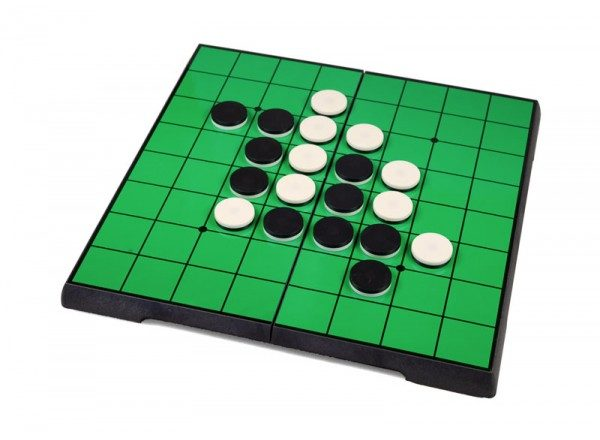
\includegraphics[width=12cm]{./sourcesIMAGES/othello.jpg}
\end{figure}

  \newpage
  \tableofcontents

  \newpage
  \section{Introduction}
    Dans le cadre du cours d'algorithmique et programattion avancée en C, notre promotion a travaillé, en groupes de4 à 5 personnes, à la réalisation d'un jeu d'Othello, entièrement développé en C. Nous avions pour cela l'aide de nos cours, des enseignants, et devions prendre l'initiative d'approfondir nos connaissances via les différents moyens à notre disposition (livres, internet), lorsque cela était nécessaire.

Nous avons réalisé ce jeu en équipe, et en suivant le cycle de développement en V, enseigné depuis la première année à l'INSA. Notre équipe est composée de 3 étudiants de STPI, un étudiant Euromed-SIC, et un étudiant intégré venant de DUT Info, tous les cinq suivant la formation ASI à l'INSA de Rouen Normandie. Avec nos approches différentes, et nos expériences plus ou moins importantes dans le domaine des projets informatiques, nous devions réussir à livrer dans les temps les dossiers et archives demandées.

  \newpage
  \section{Analyse du jeu de l'Othello}
    \subsection{Règle du jeu}
    \textbf{Plateau de jeu :}
    \begin{itemize}
        \item 64 cases (8x8)
        \item Colonne de a à h
        \item Ligne de 1 à 8 
        \item Initialiser avec deux pions noirs en e4 et d5 et deux pions blancs en d4 et e5
    \end{itemize}
    \textbf{Chaque joueur pose l'un après l'autre un pion de sa couleur}
    \begin{itemize}
        \item Obligation de capturer au moins un pion de l’adversaire
        \item Si un joueur ne peut pas capturer de pion : il passe son tour
    \end{itemize}
    \textbf{Capture de pions = retourner les pions adverses}
    \begin{itemize}
        \item Il faut placer ses pions à l'extrémité d'un alignement de pions adverses contigus terminé par un de ses propres pions (ex : B N N N N)
        \item Les alignements considérés peuvent être une colonne, une ligne, ou une diagonal
        \item Si le pion placé ferme plusieurs alignements, alors la capture des pions se fait sur tous les alignements
    \end{itemize}
    \textbf{Le jeu s'arrête quand les deux joueurs ne peuvent plus poser de pion}
    \begin{itemize}
        \item Aucun des deux joueurs ne peut jouer
        \item Le plateau ne comporte plus de case vide
    \end{itemize}
    \textbf{Score : nb de pions de sa couleur} \\ \\
    \textbf{Gagnant : le joueur ayant le score le plus grand}

\subsection{Différent mode de jeu}
    \textbf{Standard :}
    \begin{itemize}
        \item Joueur vs IA
        \item Choix de la couleur des pions que l’on donne à l’IA
    \end{itemize}
    \textbf{Tournoi :}
    \begin{itemize}
        \item Obligation de capturer au moins un pion de l’adversaire
        \item 10 secondes sur les machines des salles de TP pour jouer
        \item Communication à l’aide des entrées standards et des sorties standards du “broker”
    \end{itemize}

  \newpage
  \section{Gestion de projet}
    \hspace{3em}
La réalisation du projet, avant d’être un défi au niveau technique, se doit d’être encadrée par un ensemble de règles et d’actions pour améliorer la communication de
l’équipe et mener le projet à bien. Nous devons aussi imposer un cadre pour le développement à venir avec un ensemble de normes qu’il est important de respecter pour
garantir la clarté et donc réutilisabilité du code.


    \subsection{Règles concernant l’utilisation de git}
      \hspace{3em}
GIT est un gestionnaire de version décentralisé. C’est un outil permettant de travailler à plusieurs sur un même projet tout en permettant un suivi contribution par contribution des développeurs. En plus d’être un nouvel outil pour la majorité des membres du groupe, son utilisation peut parfois être contre intuitive. Nous avons alors organisé une petite réunion en début de projet où ceux déjà initiés (Zacharia et Alexis) ont expliqué comment il fonctionnait et ainsi défini certaines normes et bonnes pratiques à respecter.

	La première chose a été d’expliquer le fonctionnement des branches sur git. La principale étant la branche master, nous l’avons directement sécurisée en empêchant les gens d’envoyer directement leurs changements sur celle-ci. Le seul moyen de proposer des modifications est grâce aux merge request (cf partie suivante sur gitlab et son utilité). Chaque développeur tire alors une branche depuis master pour développer les fonctionnalités qu’il souhaite implémenter puis les ajoute à master une fois complétées et validées. Avoir un tel découpage permet un meilleur visuel du travail de chaque développeur et de pouvoir intervenir en cas de problèmes. De plus il permet de ne pas “abîmer” la branche master avec des commits ajoutants des erreurs inaperçues.

	Au niveau des commits nous avons également essayé de garder une unicité au niveau de leur nommage pour y faciliter la navigation. En plus d’avoir essayé au maximum de donner des noms significatifs, nous avons tenté d’appliquer un équivalent simplifié ci-dessous de la convention de nommage utilisée sur le repos git d’Angular (documentation disponible en bibliographie).

git commit -m “<type> (<scope>): <subject>”

Tout le message doit être écrit en minuscule, essayer de ne pas dépasser les 100 caractères au total. Les différents champs du message ont chacun un objectif :

\textbf{type : De quelle façon le commit modifie le projet} (1 mot exactement) parmis les suivants :
\begin{itemize}
  \item \textbf{feat} (feature = nouvelle fonctionnalité)
  \item \textbf{fix} (bug fix)
  \item \textbf{perf} (changement dans le code qui améliore les performances)
  \item \textbf{refactor} (un changement dans le code qui n’ajoute pas de fonctionnalité et ne règle pas de bug non plus)
  \item \textbf{add} (ajout d’un nouveau fichier ou de code qui ne constitue pas une fonctionnalité en soit)
  \item \textbf{test} (ajout de tests)
  \item \textbf{doc} (ajout de documentation)
  \item \textbf{style} (changement qui ne modifie pas le sens du code mais la forme, par ex parenthèses manquantes, pts virgule, …)
\end{itemize}

\textbf{scope : Sur quoi porte le commit} (entre 1 et 3 mots) par exemple :
\begin{itemize}

  \item le nom d’un fichier en particulier
  \item le nom d’un dossier
  \item une fonctionnalité en particulier
  \item une fonction en particulier
\end{itemize}

\textbf{subject : Ce que fait le commit} (max 80 caractères) par exemple :
\begin{itemize}

  \item “ajout d’une fonction de saisie d’un coup”
  \item “ajout batterie de tests sur type position”
  \item “parenthèses manquantes fonctions affichage”
\end{itemize}

\begin{center}
\textbf{On obtient alors un graphe qui a la forme suivante}
\end{center}
\begin{figure}[h]
  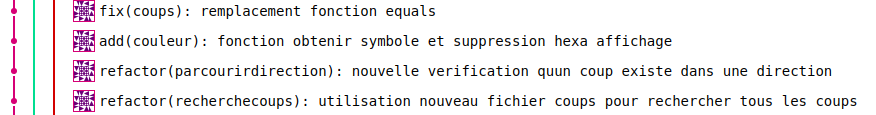
\includegraphics[width=18cm]{./sourcesIMAGES/commits.png}
  \caption{Les messages de commits sont clairs, on sait sur quoi portent les modifications}
\end{figure}


    \subsection{L'outil Gitlab et ce qu'il a permis pendant le projet}
      \hspace{3em}
Gitlab est un logiciel rendant la manipulation d’un projet utilisant git beaucoup plus simple grâce à une multitude de fonctionnalités. Nous en avons principalement utilisé deux : le gestionnaire de ticket ainsi que les merge request.

	Le gestionnaire de ticket permet d’avoir un suivi des tâches à réaliser, déjà réalisées et en cours de réalisation. Chaque chose à faire pour le projet est traduite en tâche plus ou moins atomique, certaines correspondent à un “ensemble de choses à faire” qui sont assez courtes et ont donc le même objectif. Ainsi il a été possible d’attribuer des issues (nom donné aux tickets) aux membres du groupe pour que chacun ai des choses à faire. Nous avons aussi utilisé une nomenclature pour l’écriture des issues et leur manipulation : sur leur nom, et sur leur état.

	Le nom d’une issue doit prendre la forme :

	TYPE\_ISSUE : Nom issue

Le nom de l’issue doit être assez descriptif pour que l’on comprenne à quoi elle correspond, mais assez courte car il y a un champs description justement fait pour cela.
Le type d’issue n’est pas natif dans gitlab contrairement à d’autres gestionnaires de ticket comme Jira, mais il nous a paru important d’identifier à quoi servent chaque issues.
Les types possibles sont les suivants :

\textbf{BUGFIX} : Le ticket est ouvert car une fonctionnalité présente un bug et il doit être corrigé

\textbf{FONCTIONNALITÉ} : L’issue apporte un contenu fonctionnel à l’utilisateur final (exemple : jouer une partie)

\textbf{TACHE} : L’issue doit être réalisée mais en soit elle ne présente aucun intérêt pour l’utilisateur final car lui ne verra pas le résultat (exemple : écriture de tests)

\textbf{SOUS-TACHE} : Les tâches ont parfois besoin d’être divisées en sous-tâches pour être mieux réparties entre les développeurs. La tâche correspond alors à un ensemble fonctionnel. Une sous-tâche ne peut pas elle même avoir de sous tâche. Le nom d’une issue de type sous-tâche est précédé d’un \# avec le numéro de l’issue à laquelle elle fait référence.

	L’autre utilité de Gitlab a été les merge request. Une merge request est une demande de fusion entre une branche A et une autre branche B. Ce qui veut dire que les branches A et B vont être mélangées commit par commit pour que tous les changements de la branche A soient intégrés dans la branche B.
Grâce à Gitlab les développeurs peuvent alors visionner les changements apportés par la branche A par rapport à la B, donner leur avis, et approuver la demande de merge.
Chaque développeur peut alors voir le travail fourni par les autres lorsqu’ils souhaitent proposer leurs modifications au projet, et apporter un oeil nouveau sur le travail produit. Une fois tous les commentaires validés sur la merge request, elle est prête à être “merge” directement sur la branche master.

\begin{center}
\textbf{Exemple de commentaire sur une merge request}
\end{center}
\begin{figure}[h]
  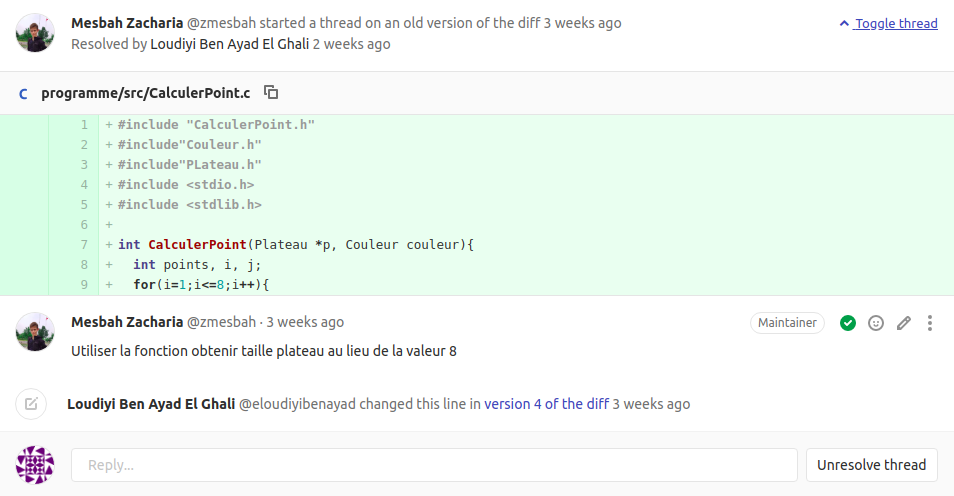
\includegraphics[width=18cm]{./sourcesIMAGES/exemple_merge_request.png}
  \caption{Ici, Zacharia fait une remarque sur un bout de code produit par El Ghali}
\end{figure}


    \subsection{Nomenclature utilisée dans le projet}
      \hspace{3em}
Dans le code en lui même nous avons aussi essayé d’appliquer des bonnes pratiques. Les plus évidentes sont le nommage explicite de fonctions et de variables, éviter au maximum les “char * tmp” et “int a,b,c” !

	Tous les fichiers .c sont accompagnés de leur fichier .h, qui est bien commenté en fonction des conventions imposées par Doxygen.

Certaines fonctions présentes dans les fichiers .c commencent par la lettre P, signifiant “privé”. Comme dans les langages orientés objets où certaines classes ont des méthodes inutilisables en dehors de cette même classe, ici nous avons fait le choix de ne pas mettre dans les .h les fonctions qui n’ont pas d’utilité en dehors du .c lui-même.

	Nous avons aussi utilisé les préfixes pour nommer les fonctions, ces préfixes font références aux types sur lesquels ils sont censés agir.

  \begin{center}
  \textbf{Exemple de fonction dans un .h}
  \end{center}
  \begin{figure}[h]
    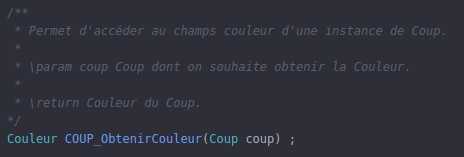
\includegraphics[width=18cm]{./sourcesIMAGES/obtenircouleur.png}
    \caption{La fonction COUP ObtenirCouleur est préfixée par COUP car c’est une action portant sur le type Coup, les commentaires utilisent des balises de Doxygen et le nom de fonction est significatif}
  \end{figure}

  Nous avons utilisé la notation en CamelCase de deux façons différentes dans notre projet. Les fonctions ont des noms avec une majuscule au tout premier mot, tandis que les variables ont une majuscule seulement à partir du second.


    \subsection{Organisation et répartition des tâches}
      \hspace{3em}
Pour lancer le projet et assurer son suivi nous avons organisé à plusieurs reprises des réunions avec les membres du groupe du projet pour parler de son avancement. Chaque membre décrivait ce qu’il avait effectué et ce qu’il lui restait à faire. C’était aussi l’occasion de revenir sur certains points faisant débat ou simplement des interrogations qui avaient besoin d’être répondues en groupe. De plus nous faisions parfois la review des merge request ensemble car les discussions sont parfois plus simples en face à face que par le système de commentaires proposé par Gitlab.

	Pour le découpage du travail chacun avait sa partie de l’analyse à effectuer et avait en général la tâche de l’implémenter en C par la suite. Les ensembles de fonctions à réaliser étaient découpés en unités logiques pour pas que les membres n’aient à faire le pseudo code de plusieurs fonctions sans rapport entre elles : celui désigné pour la partie pour jouer un coup s’occupait aussi de la capture des pions lors du dit-coup. Certains membres plus ou moins à l’aise avec le langage C ou l’analyse en général aidaient les autres dans leur tâche et parfois plusieurs personnes travaillaient sur une même fonction. L’utilité est d’avoir plusieurs versions possibles pour pouvoir choisir la meilleure (plus optimisée, plus élégante, plus simple à implémenter ?), ça a été le cas pour la fonction de recherche de tous les coups possibles pour une couleur où Jérôme et Alexis se sont penchés sur la question.


  \newpage
  \section{TADs}
    \documentclass[]{article}
\usepackage{babel}
\usepackage[utf8]{inputenc}
\usepackage{algorithmeUTF8} 
\begin{document}

	\begin{tad}
		\tadNom{Couleur}
		\tadDependances{Chaine de caractères}
		\begin{tadOperations}{Couleur}
			\tadOperation{Couleur}{\tadUnParam{Chaine de caractères}}{\tadUnParam{Couleur}}
			\tadOperation{CouleurOpposée}{\tadUnParam{Couleur}}{\tadUnParam{Couleur}}
			
		\end{tadOperations}
		\begin{tadAxiomes}
			\tadAxiome{CouleurOpposée( CouleurOpposée( Couleur ))) = Couleur}
		\end{tadAxiomes}
	\end{tad}
	
	\begin{tad}
		\tadNom{Pion}
		\tadDependances{Couleur}
		\begin{tadOperations}{Pion}
			\tadOperation{Pion}{\tadUnParam{Couleur}}{\tadUnParam{Pion}}
			\tadOperation{ObtenirCouleur}{\tadUnParam{Pion}}{\tadUnParam{Couleur}}
			\tadOperation{InverserCouleur}{\tadUnParam{Pion}}{\tadUnParam{Pion}}
		\end{tadOperations}
		\begin{tadAxiomes}
			\tadAxiome{InverserCouleur(InverserCouleur(Pion(Couleur))) = Pion}
		\end{tadAxiomes}
	\end{tad}
	
	\begin{tad}
		\tadNom{Position}
		\tadDependances{Colonne,Ligne}
		\begin{tadOperations}{Position}
			\tadOperation{Position}{\tadUnParam{Colonne x Ligne}}{\tadUnParam{Position}}
			\tadOperation{FixerColonne}{\tadUnParam{Colonne}}{\tadUnParam{Position}}
			\tadOperation{FixerLigne}{\tadUnParam{Ligne}}{\tadUnParam{Position}}
			\tadOperation{ObtenirColonne}{\tadUnParam{Position}}{\tadUnParam{Colonne}}
			\tadOperation{ObtenirLigne}{\tadUnParam{Position}}{\tadUnParam{Ligne}}
		\end{tadOperations}
		\begin{tadAxiomes}
		\end{tadAxiomes}
	\end{tad}
	
	\begin{tad}
		\tadNom{Coup}
		\tadDependances{Position,Pion,Plateau}
		\begin{tadOperations}{Coup}
			\tadOperation{Coup}{\tadUnParam{Position x Pion}}{\tadUnParam{Coup}}
			\tadOperation{ObtenirPosition}{\tadUnParam{Coup}}{\tadUnParam{Position}}
			\tadOperation{ObtenirPion}{\tadUnParam{Coup}}{\tadUnParam{Pion}}
			\tadOperation{EstValideCoup}{\tadUnParam{Plateau}}{\tadUnParam{Booleen}}
		\end{tadOperations}
		\begin{tadAxiomes}
		\end{tadAxiomes}
	\end{tad}
	
	\begin{tad}
		\tadNom{Plateau}
		\tadDependances{Position,Coup,Plateau,Pion}
		\begin{tadOperations}{Plateau}
			\tadOperation{Plateau}{\tadUnParam{Naturel x Naturel}}{\tadUnParam{Plateau}}
			\tadOperation{JouerCoup}{\tadUnParam{Plateau x Coup}}{\tadUnParam{Plateau}}
			\tadOperation{ObtenirPion}{\tadUnParam{Plateau x Position}}{\tadUnParam{Pion}}
			\tadOperation{CaseVide}{\tadUnParam{Plateau x Position}}{\tadUnParam{Booleen}}
			\tadOperation{Remplacer}{\tadUnParam{Plateau x Position}}{\tadUnParam{Plateau}}
		\end{tadOperations}
		\begin{tadAxiomes}
			\tadAxiome{ObtenirPion(JouerCoup(Plateau,Coup(Position,Pion)), Position) = Pion}
			\tadAxiome{Remplacer(Remplacer(Plateau,Position),Position) = Plateau}
		\end{tadAxiomes}
	\end{tad}
	
	\begin{tad}
		\tadNom{Coups}
		\begin{tadOperations}{Coups}
			\tadOperation{Coups}{}{\tadUnParam{Ensemble<Coup>}}
			\tadOperation{AjouterCoup}{\tadUnParam{Coups x Coup}}{\tadUnParam{Coups}}
			\tadOperation{RetirerCoup}{\tadUnParam{Coups x Coup}}{\tadUnParam{Coups}}
			\tadOperation{NombreCoups}{\tadUnParam{Coups}}{\tadUnParam{Naturel}}
		\end{tadOperations}
		
	\end{tad}
	
\end{document}

  \newpage
  \section{Analyse descendante}
    \input{./sourcesTEX/remarquesAnalyse}
    \begin{figure}[h]
  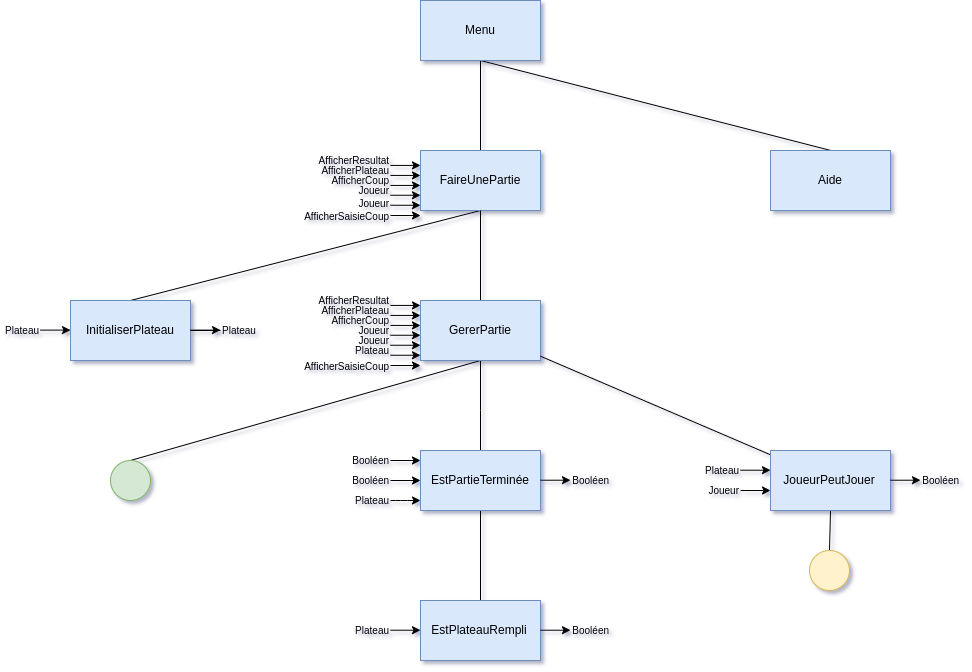
\includegraphics[width=18cm]{./sourcesIMAGES/analyse_main.png}
  \caption{Base principale de l'analyse descendante}
\end{figure}
\newpage
\begin{figure}[h]
  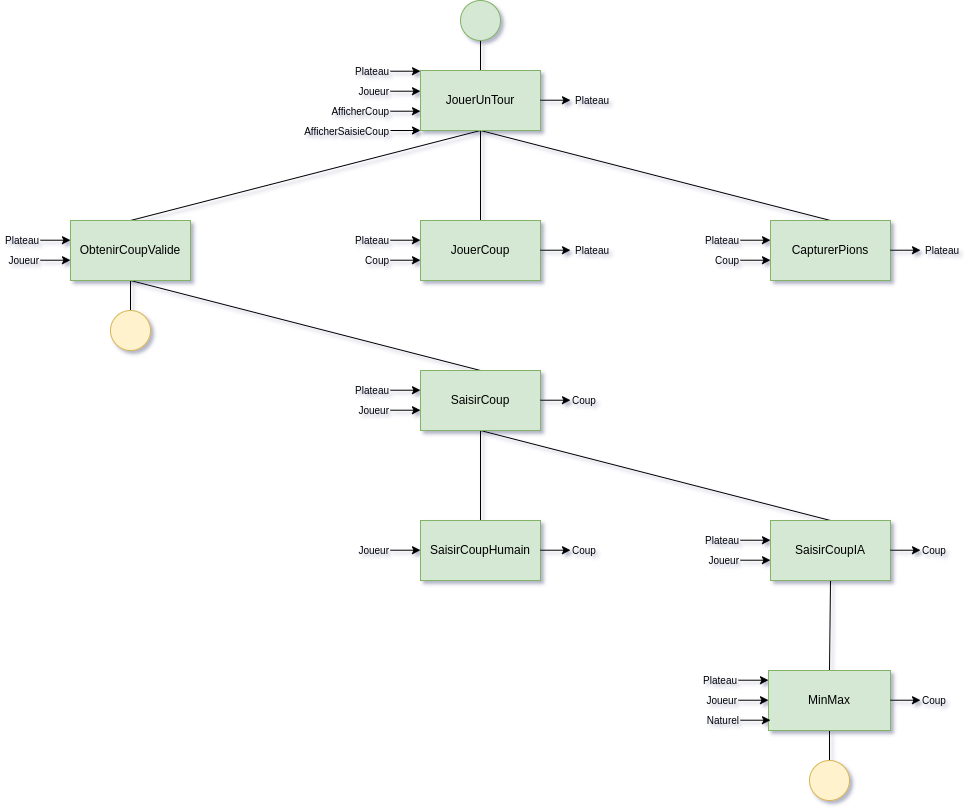
\includegraphics[width=18cm]{./sourcesIMAGES/analyse_jouerUnTour.png}
  \caption{Sous arbre de l'analyse descendante découlant de la méthode JouerUnTour}
\end{figure}
\begin{figure}[h]
  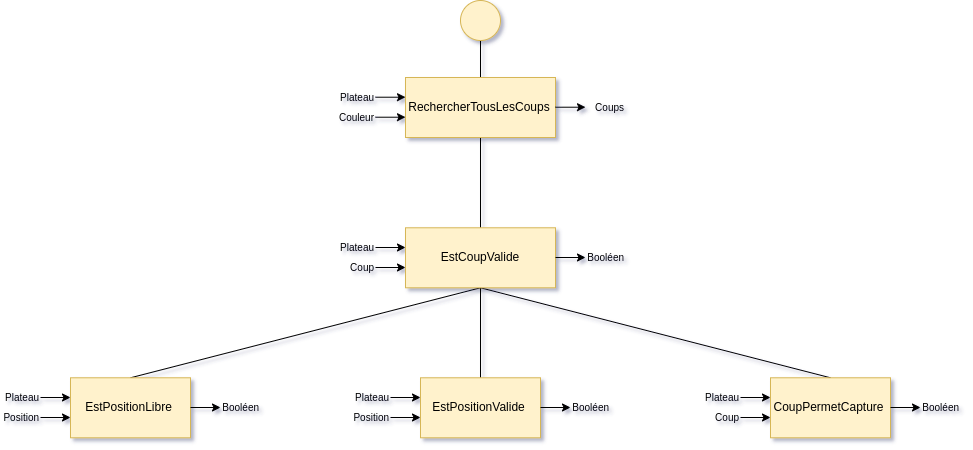
\includegraphics[width=18cm]{./sourcesIMAGES/analyse_chercherTousLesCoups.png}
  \caption{Sous arbre de l'analyse descendante découlant de la méthode RechercherTousLesCoups}
\end{figure}


  \newpage
  \section{Conception preliminaire}
       \subsection{TAD Couleur}
    \begin{algorithme}
    \signaturefonction{creerBlanc}{}{\textbf{Couleur}}
    \signaturefonction{creerNoir}{}{\textbf{Couleur}}
    \signaturefonction{creerNeutre}{}{\textbf{Couleur}}
    \signaturefonction{ObtenirCouleurOpposee}{couleur : Couleur}{\textbf{Couleur}}
    \signaturefonction{estNeutre}{}{\textbf{Couleur}}
    \signaturefonction{FixerCouleurOpposee}{couleur : Couleur, couleurOpposee : Couleur}{\textbf{Couleur}}
    \end{algorithme}
    \subsection{TAD Direction}
     \begin{algorithme}
    \signaturefonction{creerH}{}{\textbf{Direction}}
    \signaturefonction{creerHD}{}{\textbf{Direction}}
    \signaturefonction{creerD}{}{\textbf{Direction}}
    \signaturefonction{creerBD}{}{\textbf{Direction}}
    \signaturefonction{creerB}{}{\textbf{Direction}}
    \signaturefonction{creerBG}{}{\textbf{Direction}}
    \signaturefonction{creerG}{}{\textbf{Direction}}
    \signaturefonction{creerHG}{}{\textbf{Direction}}
    \signaturefonction{ObtenirDecalageColonne}{direction : Direction}{\textbf{-1},\textbf{0},\textbf{1}}
    \signaturefonction{ObtenirDecalageLigne}{direction : Direction}{\textbf{-1},\textbf{0},\textbf{1}}
    \end{algorithme}
    \subsection{TAD Etat}
     \begin{algorithme}
    \signaturefonction{creerTermine}{}{\textbf{Etat}}
    \signaturefonction{creerEnCours}{}{\textbf{Etat}}
    \signaturefonction{creerBloque}{}{\textbf{Etat}}
    \signaturefonction{EtatDeLaPartie}{plateauDeJeu : PLateau, joueurActuel : Couleur}{\textbf{Etat}}
    \end{algorithme}
    
    
    \subsection{TAD Position}
\begin{algorithme}
	\signaturefonction{CreerPosition}{c : Colonne, l : Ligne}{Position}
	\signatureprocedure{AppliquerDirection}{\paramEntreeSortie unePostion : Position, \paramEntree uneDirection : Direction}
	\signaturefonction{FixerColonne}{c : Colonne, l : Ligne}{Position}
	\signaturefonction{FixerLigne}{c : Colonne}{Position}
	\signaturefonction{ObtenirColonne}{unePostion : Position}{Colonne}
	\signaturefonction{ObtenirLigne}{unePostion : Position}{Ligne}
	\signaturefonction{EstEgalPosition}{position1, position2 : Position}{\booleen}
\end{algorithme}


\subsection{TAD Coup}
\begin{algorithme}
	\signaturefonction{CreerCoup}{unePostion : Position, uneCouleur : Couleur}{Coup}
	\signaturefonction{ObtenirPosition}{unCoup : Coup}{Position}
	\signaturefonction{ObtenirCouleur}{unCoup : Coup}{Couleur}
	\signaturefonction{EstCoupValide}{unPlateau : Plateau}{\booleen}
	\signaturefonction{EstEgalCoup}{coup1, coup2 : Coup}{\booleen}
\end{algorithme}


\subsection{TAD Coups}
\begin{algorithme}
	\signaturefonction{CreerCoups}{}{Ensemble $<$Coup$>$} \\
	Nous prendrons pour la suite :  Coups = Ensemble $<$Coup$>$
	\signaturefonction{EstVide}{lesCoups : Coups}{\booleen}
	\signatureprocedure{AjouterCoup}{\paramEntreeSortie lesCoups : Coups, \paramEntree unCoup : Coup}
	\signatureprocedure{RetirerCoup}{\paramEntreeSortie lesCoups : Coups, \paramEntree unCoup : Coup}
	\signaturefonction{ObtenirCoup}{lesCoups : Coups}{Coup}
	\signaturefonction{ObtenirNombreDeCoups}{lesCoups : Coups}{\naturel}
	\signaturefonction{EstPresent}{lesCoups : Coups, unCoup : Coup}{\booleen}
\end{algorithme}


\subsection{TAD Plateau}
\begin{algorithme}
	\signaturefonction{CreerPlateau}{}{Plateau}
	\signatureprocedure{InitialiserPlateau}{\paramEntreeSortie unPlateau : Plateau}
	\signatureprocedure{JouerCoup}{\paramEntreeSortie unPlateau : Plateau, \paramEntree unCoup : Coup}
	\signaturefonction{ObtenirCouleurAvecPosition}{unPlateau : Plateau, unePosition : Position}{Couleur}
	\signaturefonction{EstPositionLibre}{unPlateau : Plateau, unePosition : Position}{\booleen}
	\signaturefonction{ObtenirTaille}{unPlateau : Plateau}{\naturel}
	\signaturefonction{EstRempli}{unPlateau : Plateau}{\booleen}
	\signaturefonction{CalculerPoints}{unPlateau : Plateau, uneCouleur : Couleur}{\naturel}
	\signaturefonction{EstPositionValide}{unPlateau : Plateau, unePosition : Position}{\booleen}
	\signatureprocedure{CapturerPions}{\paramEntreeSortie unPlateau : Plateau, \paramEntree unCoup : Coup}
	\signatureprocedure{CapturerPionsDansDirections}{\paramEntreeSortie unPlateau : Plateau, \paramEntree unCoup : Coup, \paramEntree uneDirection : Direction}
\end{algorithme}


\subsection{TAD Ligne}
\begin{algorithme}
	\signaturefonction{ObtenirLigneDepuisInt}{ligNum : 1 .. Taille}{Ligne}
	\signaturefonction{ObtenirNumeroLigne}{l : Ligne}{1 .. Taille}
	\signaturefonction{EstEgalLigne}{l1, l2 : Ligne}{\booleen}
\end{algorithme}


\subsection{TAD Colonne}
\begin{algorithme}
	\signaturefonction{ObtenirColonneDepuisInt}{colNum : 1 .. Taille}{Colonne}
	\signaturefonction{ObtenirColonneDepuisInt}{colChar : Char}{Colonne}
	\signaturefonction{ObtenirNumeroColonne}{c : Colonne}{1 .. Taille}
	\signaturefonction{EstEgalColonne}{c1, c2 : Colonne}{\booleen}
\end{algorithme}

    \subsection{Analyse descendante bleue}	
	\begin{algorithme}
		\signaturefonction{FaireUnePartie}{AfficherResultat, AfficherPlateau, AfficherCoup, AfficherSaisieCoup : Fonction, j1, j2 : Joueur}{}
	\end{algorithme}
	\begin{algorithme}
		\signatureprocedure{InitialiserPlateau}{\paramEntreeSortie plateau : Plateau}
	\end{algorithme}
	\begin{algorithme}
		\signatureprocedure{GererPartie}{\paramEntree AfficherResultat, \paramEntree AfficherPlateau, \paramEntree AfficherCoup, \paramEntree AfficherSaisieCoup : Fonction, \paramEntree j1, \paramEntree j2 : Joueur, \paramEntreeSortie plateau : Plateau}
	\end{algorithme}
	\begin{algorithme}
		\signaturefonction{EstPartieTerminee}{plateau : Plateau, j1PeutJouer, j2PeutJouer : \booleen}{\booleen}
	\end{algorithme}
	\begin{algorithme}
		\signaturefonction{JoueurPeutJouer}{plateau : Plateau, joueur : Joueur}{\booleen}
	\end{algorithme}
	\begin{algorithme}
		\signaturefonction{EstRempli}{plateau : Plateau}{\booleen}
	\end{algorithme}
	
\subsection{Analyse descendante verte}	
	\begin{algorithme}
		\signatureprocedure{JouerUnTour}{\paramEntreeSortie plateau : Plateau, \paramEntree joueur : Joueur, \paramEntree AfficherCoup, \paramEntree AfficherSaisieCoup : Fonction}
	\end{algorithme}
	\begin{algorithme}
		\signatureprocedure{CapturerPions}{\paramEntreeSortie plateau : Plateau, \paramEntree coup : Coup}
	\end{algorithme}
	\begin{algorithme}
		\signatureprocedure{JouerCoup}{\paramEntreeSortie plateau : Plateau, \paramEntree coup : Coup}
	\end{algorithme}
	\begin{algorithme}
		\signaturefonction{ObtenirCoupValide}{plateau : Plateau, joueur : Joueur}{\textbf{Coup}}
	\end{algorithme}
	\begin{algorithme}
		\signaturefonction{SaisirCoup}{j : Joueur, plateau : Plateau}{\textbf{Coup}}
	\end{algorithme}
	\begin{algorithme}
		\signaturefonction{SaisirCoupHumain}{j : Joueur}{\textbf{Coup}}
	\end{algorithme}
	\begin{algorithme}
		\signaturefonction{SaisirCoupIA}{j : Joueur, plateau : Plateau}{\textbf{Coup}}
	\end{algorithme}
	\begin{algorithme}
		\signaturefonction{MinMax}{plateau : Plateau, joueurAMaximiser : Joueur, profondeur : \naturel}{\textbf{Coup}}
	\end{algorithme}

\subsection{Analyse descendante jaune}	
	\begin{algorithme}
		\signaturefonction{RechercherTousLesCoups}{plateauDeJeu : Plateau, couleurJoueurActuel : Couleur}{\textbf{Coups}}
	\end{algorithme}
	\begin{algorithme}
		\signaturefonction{EstCoupValide}{plateau : Plateau, coup : Coup}{\textbf{\booleen}}
	\end{algorithme}
	\begin{algorithme}
		\signaturefonction{EstPositionLibre}{plateau : Plateau, position : Position}{\textbf{\booleen}}
	\end{algorithme}
	\begin{algorithme}
		\signaturefonction{EstPositionValide}{plateau : Plateau, position : Position}{\textbf{\booleen}}
	\end{algorithme}
	\begin{algorithme}
		\signaturefonction{CoupPossibleDansUneDirectionQuelconque}{plateau : Plateau, coup : Coup}{\textbf{\booleen}}
	\end{algorithme}
	\begin{algorithme}
		\signaturefonction{CoupPossibleDansDirection}{plateau : Plateau, coup : Coup, direction : Direction}{\textbf{\booleen}}
	\end{algorithme}

  \newpage
  \section{Types}
    \input{./sourcesTEX/remarquesTypes}
    \begin{algorithme}

	\begin{enregistrement}{Couleur}
		\champEnregistrement{nom}{Chaine de caractères}
		\champEnregistrement{hexa}{Chaine de caractères}
		\champEnregistrement{couleurOpposee}{Couleur}
		\champEnregistrement{symbole}{Caractère}
		\champEnregistrement{estNeutre}{\booleen}
	\end{enregistrement}
\\
	\begin{enregistrement}{Pion [DEPRECATED]}
		\champEnregistrement{couleur}{Couleur}
	\end{enregistrement}
\\
	\begin{enregistrement}{Position}
		\champEnregistrement{ligne}{Ligne}
		\champEnregistrement{colonne}{Colonne}
	\end{enregistrement}
\\

	\begin{enregistrement}{Coup}
		\champEnregistrement{couleur}{Couleur}
		\champEnregistrement{position}{Position}
	\end{enregistrement}
\\\\
	\textbf{Type} Plateau \textbf{=} Tableau[1...Taille][1...Taille] de Couleur
\\\\
	\textbf{Type} Coups \textbf{=} Ensemble$<$Coup$>$
\\\\
	\textbf{Type} Ligne \textbf{=} 1...Taille
\\\\
	\textbf{Type} Colonne \textbf{=} 1...Taille
\\\\
	\begin{enregistrement}{Direction}
		\champEnregistrement{decalageLigne}{\{-1,0,1\}}
		\champEnregistrement{decalageColonne}{\{-1,0,1\}}
	\end{enregistrement}
\\\\
	\textbf{Type} Etat \textbf{=} {\{EN COURS, BLOQUE, TERMINE\}}


\end{algorithme}


  \newpage
  \section{Conception détaillée}
  \subsection{Analyse descendante pour faire une partie}
     \subsubsection{FaireUnePartie}
      \begin{algorithme}
	\small
	\fonction
	{FaireUnePartie}
	{joueur = Couleur, ProfondeurIA = Naturel}
	{}
	{plateau = Plateau}
	{
	\affecter{plateau}{InitialiserPlateau()}
	\tantque{non FinirLaPartie}{
		\affecter{plateau}{JouerUnTour(plateau, joueur, ProfondeurIA)}
		\affecter{joueur}{Inverser(joueur)}
	}
	}
\end{algorithme}
    \subsubsection{InitialiserPlateau}
      \begin{algorithme}
	\small
	\procedure
	{Initialiser Plateau}
	{\paramEntreeSortie p : Plateau}
	{ObtenirTaille(p) : \naturelNonNul \\
	blanc, noir, neutre : Couleur}
	{
	\affecter{neutre}{creerNeutre()}
	\affecter{blanc}{creerBlanc()}
	\affecter{noir}{creerNoir()}
	\pour{i}{1}{ObtenirTaille(p)}{}{

		\pour{j}{1}{ObtenirTaille(p)}{}{

			\instruction{JouerCoup(plateau,Coup(neutre,Position(Ligne(i),Colonne(j))))}
		}
	}

	\instruction{JouerCoup(plateau,Coup(blanc,Position(Ligne(ObtenirTaille(p) div 2),Colonne(ObtenirTaille(p) div 2))))}

	\instruction{JouerCoup(plateau,Coup(blanc,Position(Ligne(ObtenirTaille(p) div 2 + 1),Colonne(ObtenirTaille(p) div 2 + 1))))}

	\instruction{JouerCoup(plateau,Coup(noir,Position(Ligne(ObtenirTaille(p) div 2),Colonne(ObtenirTaille(p) div 2 + 1))))}

	\instruction{JouerCoup(plateau,Coup(noir,Position(Ligne(ObtenirTaille(p) div 2 + 1),Colonne(ObtenirTaille(p) div 2))))}
	}
\end{algorithme}

    \subsubsection{GererPartie}
      \begin{algorithme}
	\small
	\procedure
	{GererPartie}
	{\paramEntree AfficherResultat, \paramEntree AfficherPlateau, \paramEntree AfficherCoup : Fonction, \paramEntree j1, \paramEntree j2 : Joueur, \paramEntreeSortie plateau : Plateau}
    {j1PeutJouer, j2PeutJouer, partieTerminee : \booleen \\
    important : ChaineDeCaractères \\
    premierJoueur, secondJoueur : Joueur
    }
	{
    \affecter{j1PeutJouer}{Vrai}
    \affecter{j2PeutJouer}{Vrai}
    \affecter{partieTerminee}{Faux}
    \instruction{SetOrdreJoueurs(premierJoueur, secondJoueur, j1, j2)}
    \instruction{AfficherPlateau(plateau)}
    \tantque{non partieTerminee}{
        \affecter{j1PeutJouer}{JoueurPeutJouer(plateau, premierJoueur)}
		\sialorssinon {j1PeutJouer}{
            \instruction{JouerUnTour(plateau,premierJoueur, AfficherCoup)}
            \instruction{AfficherPlateau(plateau)}
            \affecter{partieTerminee}{EstPartieTerminee(plateau, j1PeutJouer, j2PeutJouer)}
        }
            {
            {\sialorssinon{EstIA(premierJoueur)}{
                \instruction{ecrire("passe$\backslash$n")}
            }
                {
                \instruction{lire(important)}
                }
            }
        }
        \affecter{j2PeutJouer}{JoueurPeutJouer(plateau, secondJoueur)}
		\sialorssinon {j1PeutJouer}{
            \instruction{JouerUnTour(plateau,secondJoueur, AfficherCoup)}
            \instruction{AfficherPlateau(plateau)}
        }
            {
            {\sialorssinon{EstIA(secondJoueur)}{
                \instruction{ecrire("passe$\backslash$n")}
            }
                {
                \instruction{lire(important)}
                }
            }
        }
        \affecter{partieTerminee}{EstPartieTerminee(plateau, j1PeutJouer, j2PeutJouer)}
    }
    \instruction{AfficherResultat(plateau,j1,j2)}
	}
\end{algorithme}
    \subsubsection{EstPartieTerminee}
      \begin{algorithme}
	\small
	\fonction
	{EstPartieTerminee}
	{plateau : Plateau, j1PeutJouer, j2PeutJouer : \booleen}
	{\booleen}
    {}
    {
    \sialorssinon {(non j1PeutJouer et non j2PeutJouer)}{
        \instruction{retourner Vrai}
    }{
        \sialorssinon {EstRempli(plateau)}{
            \instruction{retourner Vrai}
        }{
            \instruction{retourner Faux}
        }
    }
    }
\end{algorithme}
    \subsubsection{JoueurPeutJouer}
      \begin{algorithme}
	\small
	\fonction
	{JoueurPeutJouer}
	{plateau : Plateau, joueur : Joueur}
	{\booleen}
    {}
    {
    \sialorssinon {(ObtenirNombreDeCoups(RechercherTousLesCoups(plateau, ObtenirCouleur(joueur))) == 0)}{
        \retourner{Faux}
    }{
        \retourner{Vrai}
    }
    }
\end{algorithme}
    \subsubsection{EstRempli}
      \begin{algorithme}
	\small
	\fonction
	{EstRempli}
    {plateau : Plateau}
	{\booleen}
    {plateauEstRempli : \booleen \\
    i, j, Taille : \naturel}
    {
    \affecter{plateauEstRempli}{Vrai}
    \affecter{i}{1}
    \affecter{j}{1}
    \affecter{Taille}{ObtenirTaille(plateau)}
    \tantque{(plateauEstRempli et i < Taille)}{
        \tantque{(plateauEstRempli et j < Taille)}{
            \sialors {(EstPositionLibre(plateau, CreerPosition(i,j)))}{
                \affecter{plateauEstRempli}{Faux}
            }
            \affecter{j}{j + 1}
        }
        \affecter{i}{i + 1}
    }
    \retourner{plateauEstRempli}
    }
    \end{algorithme}

  \subsection{Analyse descendante pour jouer un tour}
    \subsubsection{JouerUnTour}
      \begin{algorithme}
	\small
	\procedure
	{JouerUnTour}
	{\paramEntreeSortie plateau : Plateau, \paramEntree joueur : Joueur, \paramEntree AfficherCoup, \paramEntree AfficherSaisieCoup : Fonction}
	{coupAJouer : Coup}
	{
	\instruction{AfficherSaisieCoup(joueur)}
	\affecter{coupAJouer}{ObtenirCoupValide(plateau, joueur)}
	\instruction{JouerCoup(plateau, coupAJouer)}
	\instruction{CapturerPions(plateau, coupAJouer)}
	\sialors{EstIA(joueur)}
		{\instruction{AfficherCoup(coupAJouer)}}
	}
\end{algorithme}
    \subsubsection{CapturerPions}
      \begin{algorithme}
	\small
	\procedure
	{CapturerPions}
	{\paramEntreeSortie plateau : Plateau, \paramEntree coup : Coup}
	{}
	{
    \instruction{CapturerPionsDansDirection(plateau, coup, H)}
    \instruction{CapturerPionsDansDirection(plateau, coup, HD)}
    \instruction{CapturerPionsDansDirection(plateau, coup, D)}
    \instruction{CapturerPionsDansDirection(plateau, coup, BD)}
    \instruction{CapturerPionsDansDirection(plateau, coup, B)}
    \instruction{CapturerPionsDansDirection(plateau, coup, BG)}
    \instruction{CapturerPionsDansDirection(plateau, coup, G)}
	\instruction{CapturerPionsDansDirection(plateau, coup, HG)}
	}
\end{algorithme}

\begin{algorithme}
	\small
	\procedure
	{CapturerPionsDansDirection}
	{\paramEntreeSortie plateau : Plateau, \paramEntree coup : Coup, \paramEntree direction : Direction}
    {nouvellePosition : Position\\
    nouveauCoup : Coup}
	{
    \sialors{(CoupPossibleDansDirection(plateau, coup, direction))}{
        \affecter{nouvellePosition}{AppliquerDirection(ObtenirPosition(coup), direction)}
        \tantque {(EstPositionValide(plateau, nouvellePosition)) et (!SontEgalesCouleurs(ObtenirCouleur(coup), ObtenirCouleurAvecPosition(plateau, nouvellePosition))))}{
            \affecter{nouveauCoup}{CreerCoup(nouvellePosition , ObtenirCouleur(coup))}
            \instruction{JouerCoup(plateau,nouveauCoup)}
            \affecter{nouvellePosition}{AppliquerDirection(ObtenirPosition(nouveauCoup), direction)}
        }
    }
	}
\end{algorithme}
    \subsubsection{JouerCoup}
      \begin{algorithme}
	\small
	\procedure
	{JouerCoup}
	{\paramEntreeSortie plateau : Plateau, \paramEntree coup : Coup}
    {positionDuCoup : Position \\
    ligneDuCoup, colonneDuCoup : \naturel \\
    coul : Couleur}
	{
	\affecter{positionDuCoup}{ObtenirPosition(coup)}
    \affecter{ligneDuCoup}{ObtenirNumeroLigne(ObtenirLigne(positionDuCoup))}
    \affecter{colonneDuCoup}{ObtenirNumeroColonne(ObtenirColonne(positionDuCoup))}
	\affecter{coul}{ObtenirCouleur(coup)}
	\affecter{plateau[(ligneDuCoup-1) * ObtenirTaille(plateau) + (colonneDuCoup-1)]}{coul}
	}
\end{algorithme}
    \subsubsection{ObtenirCoupValide}
      \begin{algorithme}
	\small
	\fonction
	{ObtenirCoupValide}
	{plateau : Plateau, joueur : Joueur}
	{Coup}
    {lesCoups : lesCoups\\
    unCoup : Coup\\
    estCoupValide : \booleen}
	{
    \affecter{lesCoups}{RechercherTousLesCoups(plateau, ObtenirCouleur(joueur))}
    \affecter{estCoupValide}{Faux}
    \tantque{non estCoupValide}{
        \affecter{unCoup}{SaisirCoup(joueur, plateau)}
        \affecter{estCoupValide}{EstPresent(lesCoups, unCoup)}
    }
    \retourner{unCoup}
	}
\end{algorithme}
    \subsubsection{SaisirCoup}
      \begin{algorithme}
	\small
	\fonction
	{SaisirCoup}
	{j : Joueur, plateau : Plateau}
	{Coup}
    {}
	{
    \sialorssinon {EstIA(j)}
    {\retourner{SaisirCoupIA(j,plateau)}}
    {\retourner{SaisirCoupHumain(j)}}
	}
\end{algorithme}
    \subsubsection{SaisirCoupHumain}
      \begin{algorithme}
	\small
	\fonction
	{SaisirCoupHumain}
	{j : Joueur}
	{Coup}
    {entree : ChaineDeCaractères\\
    ligneNombre : \naturel\\
    colonneLettre : Caractère}
	{
    \instruction{lire(entree)}
    \affecter{ligneNombre}{entree[1]}
    \affecter{colonneLettre}{entree[2]}
    \retourner{(CreerCoup(CreerPosition(ObtenirLigneDepuisInt(ligneNombre), \\ \dots \dots ObtenirColonneDepuisChar(colonneLettre)), ObtenirCouleur(j)))}
	}
\end{algorithme}
    \subsubsection{SaisirCoupIA}
      \begin{algorithme}
	\small
	\fonction
	{SaisirCoupIA}
	{j : Joueur, plateau : Plateau}
	{Coup}
    {copiePlateau : Plateau\\
    coup : Coup}
	{
    \affecter{copiePlateau}{CreerPlateau()}
    \affecter{copiePlateau}{plateau}
    \affecter{coup}{IAAlphaBeta(copiePlateau, j, j.profondeur)}
    \retourner{coup}
    }
\end{algorithme}
    \subsubsection{MinMax}
      \begin{algorithme}
	\small
	\fonction
	{MinMax}
	{plateau : Plateau, joueurAMaximiser : Joueur, profondeur : \naturel}
	{Coup}
    {coupsPossibles : Coups\\
    meilleurCoup : Coup\\
    pointsMax, resExploration : \naturel\\
    }
	{
    \affecter{coupsPossibles}{RechercherTousLesCoups(plateau,ObtenirCouleur(joueurAMaximiser))}
    \affecter{meilleurCoup}{ObtenirCoup(coupsPossibles)}
    \affecter{pointsMax}{-1}
    \tantque{(non EstVide(coupsPossibles))}
    {
        \instruction{JouerCoup(plateau, ObtenirCoup(coupsPossibles))}
        \affecter{resExploration}{IAMinMaxExplorationRecursive(joueurAMaximiser, ObtenirCouleur(joueurAMaximiser), \\.  \hspace{3cm} \dots plateau, ObtenirProfondeur(joueurAMaximiser))}
        \sialors {(resExploration > pointsMax)}
        {
            \affecter{meilleurCoup}{ObtenirCoup(coupsPossibles)}
            \affecter{pointsMax}{resExploration}
        }
        \instruction{RetirerCoup(coupsPossibles)}
    }
    \retourner{(meilleurCoup)}
	}
\end{algorithme}


  \subsection{Analyse descendante pour la recherche de tous les coups}
    \subsubsection{RechercherTousLesCoups}
      \begin{algorithme}
	\small
	\fonction
	{rechercherTousLesCoups}
	{plateauDeJeu : Plateau, joueurActuel : Couleur}
	{Coups}
	{lesCoups : Coups \\
	i : 1 .. Taille \\
	j : 1 .. Taille}
	{
	\pour{i}{1}{Taille}{}{
		\pour{j}{1}{Taille}{}{
			\sialors {rechercherUnCoup (plateauDeJeu, joueurActuel, Position(i,j))}
				{\instruction{ajouterCoup (lesCoups, coup(Position(i,j), joueurActuel)}}
		}
	}
	\retourner{(lesCoups)}
	}
\end{algorithme}

\vspace*{2cm}

\begin{algorithme}
	\small
	\fonction
	{rechercherUnCoup}
	{plateauDeJeu : Plateau, joueurActuel : Couleur, positionDuCoup : Position}
	{\booleen}
	{}
	{
	\sialorssinon {EstPositionVide (plateauDeJeu, positionDuCoup)}
			{\retourner{parcourirLesDirections (unPlateauDeJeu, positionDuCoup, joueurActuel)}}
			{\retourner{(Faux)}}		
	}
\end{algorithme}

\vspace*{2cm}

\begin{algorithme}
	\small
	\fonction
	{parcourirLesDirections}
	{unPlateauDeJeu : Plateau, positionDuCoup : Position, joueurActuel: Couleur}
	{\booleen}
	{}
	{
	\retourner{parcourirUneDirection (unPlateauDeJeu, positionDuCoup, HG, joueurActuel)\\
	ou (parcourirUneDirection (unPlateauDeJeu, positionDuCoup, H, joueurActuel)\\
	ou (parcourirUneDirection (unPlateauDeJeu, positionDuCoup, HD, joueurActuel)\\
	ou (parcourirUneDirection (unPlateauDeJeu, positionDuCoup, D, joueurActuel)\\
	ou (parcourirUneDirection (unPlateauDeJeu, positionDuCoup, BD, joueurActuel)\\
	ou (parcourirUneDirection (unPlateauDeJeu, positionDuCoup, B, joueurActuel)\\
	ou (parcourirUneDirection (unPlateauDeJeu, positionDuCoup, BG, joueurActuel)\\
	ou (parcourirUneDirection (unPlateauDeJeu, positionDuCoup, G, joueurActuel)}
	}
\end{algorithme}

\vspace*{2cm}

\begin{algorithme}
	\small
	\fonction
	{parcourirUneDirection}
	{unPlateauDeJeu : Plateau, positionDuCoup : Position, uneDirection : Direction, joueurActuel : Couleur}
	{\booleen}
	{ligneEnCours, directionValide : \booleen \\
	i : 1 .. Taille\\
	j : 1 .. Taille}
	{
	\affecter{i}{obtenirNumeroLigne (positionDuCoup)}
	\affecter{j}{obtenirNumeroColonne (positionDuCoup)}
	\affecter{ligneEnCours}{Faux}
	\affecter{directionValide}{Faux}
	\instruction{appliquerDirection (positionDuCoup, uneDirection)}
	\sialors{obtenirCouleur (unPlateauDeJeu, positionDuCoup) $\neq$ joueurActuel}{
		\affecter{ligneEnCours}{Vrai}
		\tantque{(non directionValide et ligneEnCours)}{
			\instruction{appliquerDirection (positionDuCoup, uneDirection)}
			\sialorssinon {EstPositionVide (plateauDeJeu, positionDuCoup)}
				{\affecter{ligneEnCours}{Faux}}
				{\sialors{obtenirCouleur (unPlateauDeJeu, positionDuCoup) = joueurActuel}
					{\affecter{directionValide}{Vrai}}}
		}
	}
	\retourner{(directionValide)}
	}
\end{algorithme}
    \subsubsection{EstUnCoupValide}
      \begin{algorithme}
	\small
	\fonction
	{EstUnCoupValide}
	{coupAJouer : Coup, coupsPossibles : Coups, p : Plateau}
	{\booleen}
	{
	\retourner{EstPresent(coupsPossibles,coupAJouer) and ObtenirLigne(ObtenirPosition(coupAJouer)) <= ObtenirTaille(p) and ObtenirColonne(ObtenirPosition(coupAJouer)) <= ObtenirTaille(p) and EstPositionVide(p,ObtenirPosition(coupAJouer))}
	}
\end{algorithme}
    \subsubsection{EstPositionLibre}
      \begin{algorithme}
	\small
	\fonction
	{EstPositionLibre}
	{plateau : Plateau, position : Position}
	{\booleen}
    {couleurDeLaCase : Couleur}
	{
    \affecter{couleurDeLaCase}{ObtenirCouleurAvecPosition(plateau, position)}
    {\retourner{(SontEgalesCouleurs(couleurDeLaCase, ObtenirCouleurNeutre()))}}
	}
\end{algorithme}
    \subsubsection{EstPositionValide}
      \begin{algorithme}
	\small
	\fonction
	{EstPositionLibre}
	{plateau : Plateau, position : Position}
	{\booleen}
    {colonne : Colonne\\
    ligne : Ligne}
	{
    \affecter{colonne}{ObtenirColonne(position)}
    \affecter{ligne}{ObtenirLigne(position)}
    {\retourner{((ObtenirNumeroColonne(colonne) $\leq$ ObtenirTaille(plateau)) \\ \dots \dots
     et (ObtenirNumeroLigne(ligne) $\leq$ ObtenirTaille(plateau)) \\ \dots \dots
     et (ObtenirNumeroColonne(colonne) $\geq$ 1) et (ObtenirNumeroLigne(ligne) $\geq$ 1))}}
	}
\end{algorithme}
    \subsubsection{CoupPermetCapture}
      \begin{algorithme}
	\small
	\fonction
	{CoupPossibleDansUneDirectionQuelconque}
	{plateau : Plateau, coup : Coup}
	{\booleen}
	{}
	{
    \retourner{CoupPossibleDansDirection(plateau, coup, HG) \\ \dots
    ou CoupPossibleDansDirection(plateau, coup, H)\\ \dots
    ou CoupPossibleDansDirection(plateau, coup, HD)\\ \dots
    ou CoupPossibleDansDirection(plateau, coup, D)\\ \dots
    ou CoupPossibleDansDirection(plateau, coup, BD)\\ \dots
    ou CoupPossibleDansDirection(plateau, coup, B)\\ \dots
    ou CoupPossibleDansDirection(plateau, coup, BG)\\ \dots
    ou CoupPossibleDansDirection(plateau, coup, G)}
	}
\end{algorithme}

\vspace*{1cm}

\begin{algorithme}
	\small
	\fonction
	{CoupPossibleDansDirection}
	{plateau : Plateau, coup : Coup, direction : Direction}
	{\booleen}
    {nouvellePosition : Position\\
    caseVideRencontree, maCouleurRencontree, limitePlateauAtteinte  : \booleen}
	{
    \affecter{nouvellePosition}{AppliquerDirection(ObtenirPosition(coup), direction)}
    \sialors{(non EstPositionValide(plateau, nouvellePosition))}
        {\retourner{Faux}}
    \sialors{(non SontEgalesCouleurs(ObtenirCouleurAvecPosition(plateau, nouvellePosition), \\\dots \dots ObtenirCouleurOpposee(ObtenirCouleur(coup))))}
        {\retourner{Faux}}
    
    \affecter{caseVideRencontree}{Faux}
    \affecter{maCouleurRencontree}{Faux}
    \affecter{limitePlateauAtteinte}{Faux}
    \tantque{(non caseVideRencontree et non maCouleurRencontree et non limitePlateauAtteinte)}
        {
            \affecter{nouvellePosition}{AppliquerDirection(nouvellePosition, direction)}
            \affecter{limitePlateauAtteinte}{non EstPositionValide(plateau, nouvellePosition)}
            \sialors{non limitePlateauAtteinte}
            {
                \sialorssinon{(SontEgalesCouleurs(ObtenirCouleurAvecPosition(plateau, nouvellePosition), ObtenirCouleur(coup)))}
                {
                    \affecter{maCouleurRencontree}{Vrai}
                }
                {
                    \sialors{(EstPositionLibre(plateau, nouvellePosition))}
                    {\affecter{caseVideRencontree}{Vrai}}
                }
            }
        }
	\retourner{(maCouleurRencontree)}
	}
\end{algorithme}

  \newpage
  \section{Développement en C}
    \hspace{3em}Lors de l’analyse nous imaginions avoir le TAD “Coups” sous la forme d’un ensemble, car il n’y a jamais de doublon dans une liste de Coups et les opérations des ensembles nous semblaient idéales. Cependant n'ayant pas trouvé de bibliothèque intégrant les Ensembles en C (il y en avait une qui proposait des ensembles de Strings, après réflexion nous aurions pu l’utiliser en ayant 2 fonctions qui permettent d’encoder et décoder un Coup en un String, mais faute de temps nous ne l’avons pas implémenté). 

Nous sommes alors partis sur une conception avec des Listes Chaînées où le Noeud comportait un Coup et un pointeur vers un autre Noeud. Cela semblait une bonne alternative, en plus d’apporter une optimisation au niveau de la gestion de la mémoire. Nous avons alors travaillé très longtemps avec un type Liste Chainées que nous avions écrit entièrement nous même. Malheureusement, leur manipulation s’est révélée être un calvaire à cause de nombreux bugs. Léo Pacary est alors venu à notre rescousse et nous a aidé avec un type Coups qu’il avait lui même codé et qui était infiniment plus simple et efficace, nous avons alors fait le choix de le citer dans le code source en tête de fichier et de le mentionner ici en remerciements.

    \subsection{Dossier /src}
    \lstinputlisting{../programme/src/Affichage.c}
    \newpage
    %\lstinputlisting{../programme/src/Aide.c}
    %\newpage
    \lstinputlisting{../programme/src/Colonne.c}
    \newpage
    \lstinputlisting{../programme/src/Couleur.c}
    \newpage
    \lstinputlisting{../programme/src/Coup.c}
    \newpage
    \lstinputlisting{../programme/src/Coups.c}
    \newpage
    \lstinputlisting{../programme/src/Direction.c}
    \newpage
    \lstinputlisting{../programme/src/GererPartie.c}
    \newpage
    \lstinputlisting{../programme/src/IntelligenceArtificielle.c}
    \newpage
    \lstinputlisting{../programme/src/Joueur.c}
    \newpage
    \lstinputlisting{../programme/src/Ligne.c}
    \newpage
    \lstinputlisting{../programme/src/Menu.c}
    \newpage
    \lstinputlisting{../programme/src/MenuGraphique.c}
    \newpage
    \lstinputlisting{../programme/src/MenuLigneCommande.c}
    \newpage
    \lstinputlisting{../programme/src/Othello.c}
    \newpage
    \lstinputlisting{../programme/src/Parcourir_Direction.c}
    \newpage
    \lstinputlisting{../programme/src/Plateau.c}
    \newpage
    \lstinputlisting{../programme/src/Position.c}
    \newpage
    \lstinputlisting{../programme/src/Recherche_Coup.c}
    \newpage

\subsection{Dossier /include}
    \lstinputlisting{../programme/include/Affichage.h}
    \newpage
    %\lstinputlisting{../programme/include/Aide.h}
    %\newpage
    \lstinputlisting{../programme/include/Colonne.h}
    \newpage
    \lstinputlisting{../programme/include/Couleur.h}
    \newpage
    \lstinputlisting{../programme/include/Coup.h}
    \newpage
    \lstinputlisting{../programme/include/Coups.h}
    \newpage
    \lstinputlisting{../programme/include/Direction.h}
    \newpage
    \lstinputlisting{../programme/include/GererPartie.h}
    \newpage
    \lstinputlisting{../programme/include/IntelligenceArtificielle.h}
    \newpage
    \lstinputlisting{../programme/include/Joueur.h}
    \newpage
    \lstinputlisting{../programme/include/Ligne.h}
    \newpage
    \lstinputlisting{../programme/include/Menu.h}
    \newpage
    \lstinputlisting{../programme/include/MenuGraphique.h}
    \newpage
    \lstinputlisting{../programme/include/MenuLigneCommande.h}
    \newpage
    \lstinputlisting{../programme/include/Othello.h}
    \newpage
    \lstinputlisting{../programme/include/Parcourir_Direction.h}
    \newpage
    \lstinputlisting{../programme/include/Plateau.h}
    \newpage
    \lstinputlisting{../programme/include/Position.h}
    \newpage
    \lstinputlisting{../programme/include/Recherche_Coup.h}
    \newpage

\subsection{Dossier /tests}
    % \lstinputlisting{../programme/tests/testAffichage.h}
    \lstinputlisting{../programme/tests/testAffichage.c}
    \newpage
    \lstinputlisting{../programme/tests/testCalculerPoint.h}
    \lstinputlisting{../programme/tests/testCalculerPoint.c}
    \newpage
    \lstinputlisting{../programme/tests/testColonne.h}
    \lstinputlisting{../programme/tests/testColonne.c}
    \newpage
    \lstinputlisting{../programme/tests/testCouleur.h}
    \lstinputlisting{../programme/tests/testCouleur.c}
    \newpage
    \lstinputlisting{../programme/tests/testCoup.h}
    \lstinputlisting{../programme/tests/testCoup.c}
    \newpage
    \lstinputlisting{../programme/tests/testCoups.h}
    \lstinputlisting{../programme/tests/testCoups.c}
    \newpage
    \lstinputlisting{../programme/tests/testJouerCoup.h}
    \lstinputlisting{../programme/tests/testJouerCoup.c}
    \newpage
    \lstinputlisting{../programme/tests/testLigne.h}
    \lstinputlisting{../programme/tests/testLigne.c}
    \newpage
    \lstinputlisting{../programme/tests/testObtenirCoupJoueur.h}
    \lstinputlisting{../programme/tests/testObtenirCoupJoueur.c}
    \newpage
    \lstinputlisting{../programme/tests/testParcourirLesDirections.h}
    % \lstinputlisting{../programme/tests/testParcourirLesDirections.c}
    \newpage
    \lstinputlisting{../programme/tests/testParcourirUneDirection.h}
    % \lstinputlisting{../programme/tests/testParcourirUneDirection.c}
    \newpage
    \lstinputlisting{../programme/tests/testPlateau.h}
    \lstinputlisting{../programme/tests/testPlateau.c}
    \newpage
    \lstinputlisting{../programme/tests/testRechercheDesCoups.h}
    \lstinputlisting{../programme/tests/testRechercheDesCoups.c}
    \newpage
    \lstinputlisting{../programme/tests/TypesTest.h}
    \lstinputlisting{../programme/tests/TypesTests.c}
    \newpage
    

  \newpage
  \section{Bilan et Conclusion}
    <<<<<<< HEAD
\hspace{3em}

Finalement nous avons réussi à obtenir un jeu d’Othello fonctionnel et respectant beaucoup des exigences : affichage de l’aide, jouable en mode joueur contre joueur, standard contre une IA, et en mode tournoi avec le script proposé. Nous avons également ajouté la possibilité de lancer le jeu avec un menu, certes assez sommaire, mais qui permet de lancer une partie différemment qu’en ligne de commande.

Pour revenir sur le déroulement de ce projet nous pensons globalement que cela s’est bien déroulé même si nous avons eu quelques soucis pour le respect des délais. Il aurait été évidemment possible d’améliorer le résultat en ayant plus de rigueur dans le développement et en respectant encore plus les bonnes pratiques que nous nous sommes imposé.

Plusieurs améliorations sont possibles mais nous en avons clairement identifié certaines qui sont les suivantes : la fonction rechercherTousLesCoups est utilisée à plusieurs endroits notamment pour la validité d’un coup et pourrait être appelée une seule fois puis l’argument passé de fonctions en fonctions. Il est aussi possible d’améliorer l’affichage du plateau et l’interface utilisateur, même si le C est rarement fait pour ça il existe des bibliothèques le permettant. L’intelligence artificielle a aussi bien besoin d’être améliorée car nous n’avons pas réussi à identifier d’où venait le problème qui faisait que l’IA joue toujours quasiment instantanément même à une grande profondeur.



En conclusion ce projet a permis de découvrir ce qu’était un projet d’informatique en groupe pour certains, et d’approfondir leurs connaissances pour d’autres. Les bases de chacun en C ont été consolidées par la partie développement et les compétences en conception d’application améliorées par la partie Analyse.
=======
\begin{tabular}{|*{6}{c|}}
    \hline
   	Cycle  & Ben Ayad El Ghali  & Melo Alexis  & Mesbah Zacharia  & Saivres Jérôme  & Si Ruixu \\
    \hline
    Analyse  & 5h00  & 5h00  & 5h00  &  5h00  & 5h00  \\
    \hline
   	Conception Préliminaire & 3h00  & 3h00  & 3h00  & the rest & 1h30 \\
    \hline
   	Conception Détaillée & 3h30  & 10h00  & 6h00  & 20h00  & 2h30 \\
    \hline
   	 Developpement & 4h00  & 40h00  &  70h00 & 6h00  & 5h30 \\
    \hline
   	 Test Unitaire  &js  & 1h00  & 10h00  & 8h00 & 1h00 \\
    \hline
   	 Reunion  & 7h00  & 7h00  & 7h00  & 7h00 & 7h00 \\
    \hline
   	 Gestion de projet & -- & 10h00  & --  & -- & -- \\
    \hline
\end{tabular}
>>>>>>> 82274205c2331319642ef2ceac7451240ca07dc8


\end{document}
